\documentclass{article}

%%%%%%%%%%%%%%%%%
%    Packages   %
%%%%%%%%%%%%%%%%%

\usepackage{amsmath}
\usepackage{mathtools}
\usepackage{cancel}
\usepackage{amsfonts}
\usepackage{amssymb}
\makeatletter
\def\amsbb{\use@mathgroup{}\M@U{}\symAMSb}
\makeatother
\usepackage{bbold}
\usepackage{mathabx}
\usepackage{stmaryrd}
\usepackage{graphicx}
\usepackage{amssymb}
\usepackage{float}
\usepackage{enumitem}
\usepackage{mdframed}
\usepackage{tikz}
\usetikzlibrary{decorations.markings,arrows,decorations.pathreplacing}
\usetikzlibrary{arrows}
\usetikzlibrary{automata,positioning}
\usepackage{mathrsfs}
\usepackage[top=0.8in, bottom=0.8in, left=0.7in, right=0.7in]{geometry}
\usepackage{color}
\usepackage{dsfont}
\usepackage{bold-extra}
\usepackage{lastpage}
\usepackage{fancyhdr}
\usepackage{algorithmic}
\usepackage[]{algorithm2e} %lined,boxed, linesnumbered, ruled
\usepackage{listings}
\usepackage{wrapfig}

%%%%%%%%%%%%%%%%%%
%      CODE      %
%%%%%%%%%%%%%%%%%%

% CODE %
\definecolor{gray}{rgb}{0.5,0.5,0.5}
\definecolor{purple}{HTML}{BF0EB3}

\lstset{frame=tb,
	language=C,
	aboveskip=3mm,
	belowskip=3mm,
	showstringspaces=false,
	columns=flexible,
	basicstyle={\small\ttfamily},
	numbers=none,
	numberstyle=\tiny\color{purple},
	keywordstyle=\color{blue},
	commentstyle=\color{gray},
	stringstyle=\color{red},
	breaklines=true,
	breakatwhitespace=true,
	tabsize=3
}

% example custom highlighting
%\lstset{emph={%  
%	LOAD, SAVE, string%
%	},emphstyle={\color{blue}}%
%}% 

% example DFA drawing
% \begin{tikzpicture}[shorten >=1pt,node distance=2cm,on grid,auto] 
%    \node[state,initial] (q_0)   {$q_0$}; 
%    \node[state] (q_1) [above right=of q_0] {$q_1$}; 
%    \node[state] (q_2) [below right=of q_0] {$q_2$}; 
%    \node[state,accepting](q_3) [below right=of q_1] {$q_3$};
%     \path[->] 
%     (q_0) edge  node {0} (q_1)
%           edge  node [swap] {1} (q_2)
%     (q_1) edge  node  {1} (q_3)
%           edge [loop above] node {0} ()
%     (q_2) edge  node [swap] {0} (q_3) 
%           edge [loop below] node {1} ();
% \end{tikzpicture}

\begin{document}

\subsection*{Features}
For the calculation of $Y2$, the following features were considered.

\begin{itemize}
    \item Age: The age of the athlete in 2016. This was estimated by finding the upper and lower bounds of the athlete's age
                based on the dates of past races and the category the runner was in for that race.
    \item Sex: Taken from the categories of the runner. (represented as 0 for female and 1 for male)
    \item Average distance run: The average distance of running events the in which athlete has participated.
    \item Timeweight: % TODO: Shi Yan, wanna explain this? 
    \item Average speed: Average speed of running events.
    \item Speed$^2$: The average speed squared.
    \item Speed$^{-1}$: One over the average speed. 
    \item 5k speed:  Average speed for 5k events. 
    \item 10k:  Average speed for 10k events.
    \item Half Marathon:  Average speed for half marathon events.
    \item Marathon: Average speed for for marathon events.
    \item Finishing ratio:  The ratio of events finished to events in which the runner participated. 
\end{itemize}

We represented each runner as an object so that each team member could easily and independently
develop features as methods.

\subsection*{Linear Regression Training Method}

A test set was put aside to allow us to attempt to evaluate what our performance will be with unseen data. 

The linear regression used the closed form matrix solution. This method was chosen primarily for simplicity. 
Given that the data set is not too large for a laptop to evaluate matrix multiplications and that it seems quite 
unlikely that two rows would, we concluded that the closed form solution is reasonable.

Given the number of features we have, versus the size of the data set, we decided against regularization.

In order to have a labeled set on which we could do a regression, we used all runners who had participated in the 2015 marathon,
taking their time in the 2015 marathon as a label and removing this data point from all feature calculations. 
In the event that a runner didn't finish the marathon, they were given a time of -1.

In order to determine which features would provide the best results, we tried all possible combinations
of the features listed above. In order to finish the project on time, this process was paralellized using 
the python multiproccessing library for increased performance.

To evaluate a set of features, $10$-fold validation was used. The set of features which showed the smallest
average total squared error were: Marathon, Half marathon, 10k, Finishing ratio, Age and Timeweight.

Using these features, all the data (test set included) were used to train a function based on these features.

This function was then evaluated on all data to create our predictions. In the event that an athete was missing a feature (due to lack of data),
we used a $0$ in that feature's place.


\subsection*{Linear Regression Results}


We evaluated error on a set by calculating the average number of seconds by which we were off 
from the true result.
On the training set, we acheived an error of , while on the validation set we acheived an error of .
The inherent issue with this method is that we cannot be certain of the error for those who did not compete 
in the 2015 marathon (which we could conceivably see being higher, since only those that did compete
are included in the training set). However, we did not find a simple way to counteract this.

%In order to visually evaluate our performace, we did a principal component analysis on the data.
%By finding the eigen

See Table~\ref{tbl:predtrain} and Table~\ref{tbl:predvalid} where we show a random selection of 
runners from both our training set and validation set and compare their running times to our predicted running times. 


\begin{table}[ht!]
    \centering
    \begin{tabular}{| l | l | l |}
        \hline
        {\em Runner ID} & {\em Predicted Time} & {\em Actual Time}  \\ \hline
        0 & 0 & 0  \\ \hline
    \end{tabular}
    \caption{Sample predictions for the training set}
    \label{tbl:predtrain}
\end{table}

\begin{table}[ht!]
    \centering
    \begin{tabular}{| l | l | l |}
        \hline
        {\em Runner ID} & {\em Predicted Time} & {\em Actual Time}  \\ \hline
        0 & 0 & 0  \\ \hline
    \end{tabular}
    \caption{Sample predictions for the validation set}
    \label{tbl:predvalid}
\end{table}




\subsection*{Linear Regression Discussion}

A large part of the effort went into which features our report would feature. A sample regression was done using only
one feature, in an attempt to gain some intuition about which features best described the finishing times.
Some initial plots can be found in Appendix A.

A few sample results from the process of choosing features are included in Appendix B.
In addition to determining which combination of features provided the best results, various modifications of
the procedure were tried. These included replacing 0 for female and 1 for male with -1 for female and 1 for male and not
subtracting the means from the data, and only subtracting the means from continuous features (i.e.\ not subtracting 
the mean from the finishing ratio, sex, or timeweight). 
We chose the method which yielded the best results in cross validation. 

In the event that a runner was missing data for one or more features, we were faced with a choice of either excluding the
runner for the training set, or placing a $0$ (or $-1$) in the place of said feature. The results were marginally better (see the Table~\ref{tbl:avgerrs}) when 
the runner was excluded from training set, which brought about the idea for a possible improvment.

\begin{table}[ht!]
    \centering
    \begin{tabular}{| l | l |}
        \hline
        {\em Method} & {\em Average Error (seconds)}  \\ \hline
        Runners without features filtered &   \\ \hline
        0 inserted for default when a feature is missing &   \\ \hline
        -1 inserted for default when a feature is missing &  \\ \hline
    \end{tabular}
    \caption{Average errors for different strategies}
    \label{tbl:avgerrs}
\end{table}


Instead of having one linear function for a selected set of features, why not store the function for all combinations
and then, given a runner, choose the combination of features for which the runner has data that gave the best results.
For example, say we have one model $A$, based on age, 10k time and half marathon time, and a second worse model $B$ based
on age, marathon time and average distance. Given a runner who has never run a 10k, but has run a marathon, we would
evaluate them on model $B$ simply because, despite $B$ being a worse model, we at least are not artifically forcing some features
to 0. 

This approach seemed attractive to us, because setting missing data to 0 seems as though it may introduce bias (giving speed$^{-1}$ a value
of 0 seems to suggest the runner was very fast, rather than actually not having run anything), however, given the
added complexity for implementation and the computational costs for computing a model for all feature combinations
each time we make predictions, as well as the minimal difference in errors for when we artificially insert $0$ in features,
we decided against this approach.

% TODO
%Having set aside one fifth of our data as an untouched validation set in the begining, we're in a good position to
%estimate our performance on the test set. Given that our average error on our validation set is around 10 minutes,
%we're optimistic we will have similar results on the test set.


\subsection*{Appendix A}

Some sample plots of regression done on individual features.

\begin{figure}[ht!]
\centering
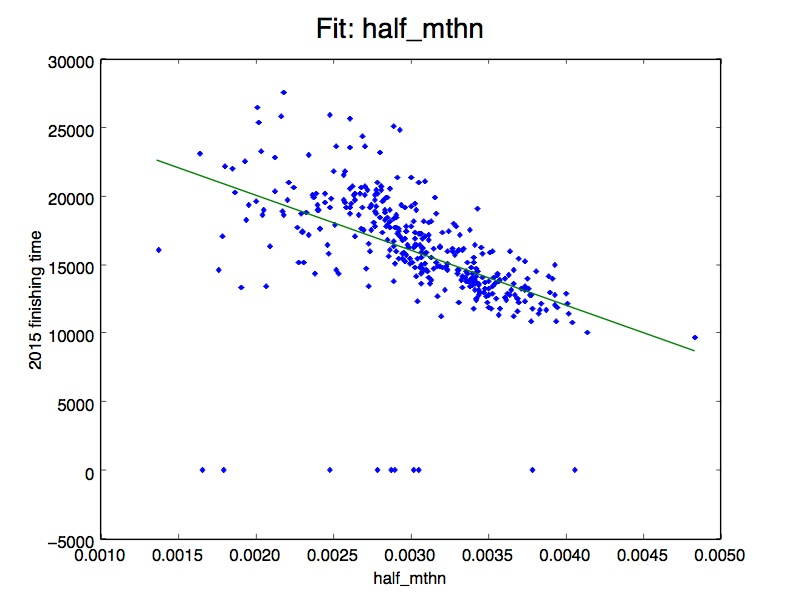
\includegraphics[width=0.8\textwidth]{half_mthn.jpg}
\caption{Half marathon time seems to be a good indicator on it's own}
\label{fig:halfmthntime}
\end{figure}

\begin{figure}[ht!]
\centering
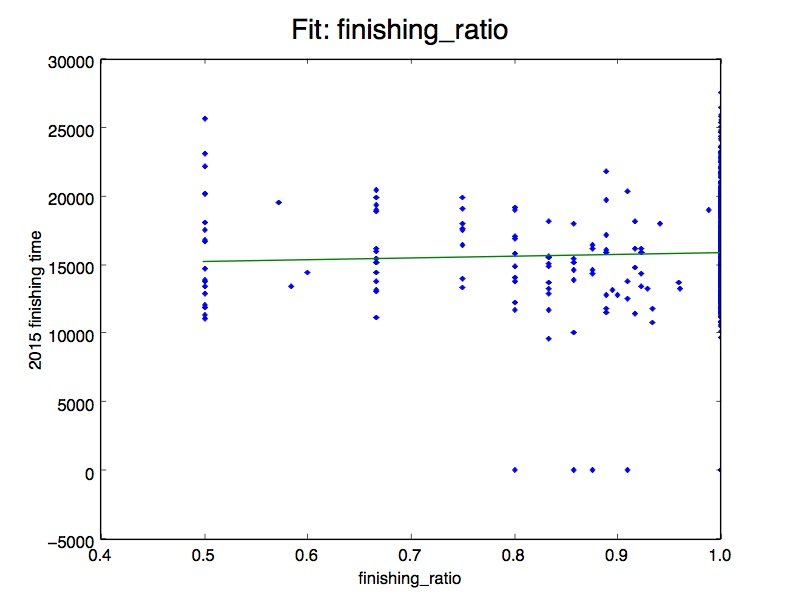
\includegraphics[width=0.8\textwidth]{finishing_ratio.jpg}
\caption{The trend in finishing ratio is less clear}
\label{fig:frtime}
\end{figure}

\subsection*{Appendix B}

A table of average errors for different feature combinations

\begin{table}[ht!]
    \centering
    \begin{tabular}{| l | l |}
        \hline
        {\em Features} & {\em Average Error (seconds)}  \\ \hline
    \end{tabular}
    \caption{Average errors for different strategies}
    \label{tbl:avgerrs}
\end{table}

\end{document}

